\chapter{系統架構與方法}
\label{chapter:system}



\section{系統架構}
\label{sec:systemarchi}
本研究專注於透過設計資料庫並用其資料訓練夾取可行性預測系統,並以此作為線索作為雙手臂主動式操作系統的策略因此可分為三大部分:商品語意基準資料庫、夾取可行性預測系統、雙手臂主動式操作系統。基準資料庫目的在設計一個專門給日常商品的資料庫,此資料庫包含物品場景圖片、商品語意如商品整體遮罩、條碼遮罩、品牌文字遮罩,因此可利用這份資料集訓練夾取可行性預測系統,基準資料庫包含參考Amazon Picking Challenge來選取物品、實驗環境設計、並分別搭建現實與虛擬環境以蒐集資料並加以驗證。而夾取可行性預測系統則是改善~\cite{peterthesis}所提出之商品文字姿態估計系統之缺點,並改良成雙手臂夾取可行性預測系統,此系統包含品牌文字、物品語意分割、以及基於語意與三維點雲資訊之夾取可行性預測。而最後的雙手臂主動式操作系統則是設計雙手臂協作方式、手臂功能、假爪選擇與設計、以及最後執行任務之有限狀態機(Finite State Machine)。此系統的設計考量與基準資料庫物品選擇、夾取可行性預測系統環環相扣,因此接下來將先說明環境架設以及主動式操作系統硬體設計,接下來依序說明如何蒐集商品語意基準資料庫、夾取可行性預測系統。最後以主動式操作系統有限狀態機總結整體系統。

\section{硬體架構與工作環境配置}
本研究提出的系統建立在兩隻協作型手臂上。一為協作手臂UR5,並裝上Robotiq 2F-85雙指假爪作為末端效應器以及RGB-D深度攝影機Realsense SR300,另一隻手臂則是則是UR3,並裝上自製的吸盤假爪。這兩隻手臂被固定在同一張桌上,並彼此距離1公尺。此外,桌上有兩個盒子在手臂之間,一個盒子是被裝滿物品的,而另一個而是空的。裝滿物體的盒子上有配置深度攝影機,作為觀察盒子物體用。整個系統會從充滿物品的盒子開始:UR3把物體從雜亂的盒子中取出,並放到空盒或停留於空中作為暫時位置,等待UR5夾取並以特定姿勢擺放至架上固定的格子裡。

\begin{figure}[ht]
	\centering
	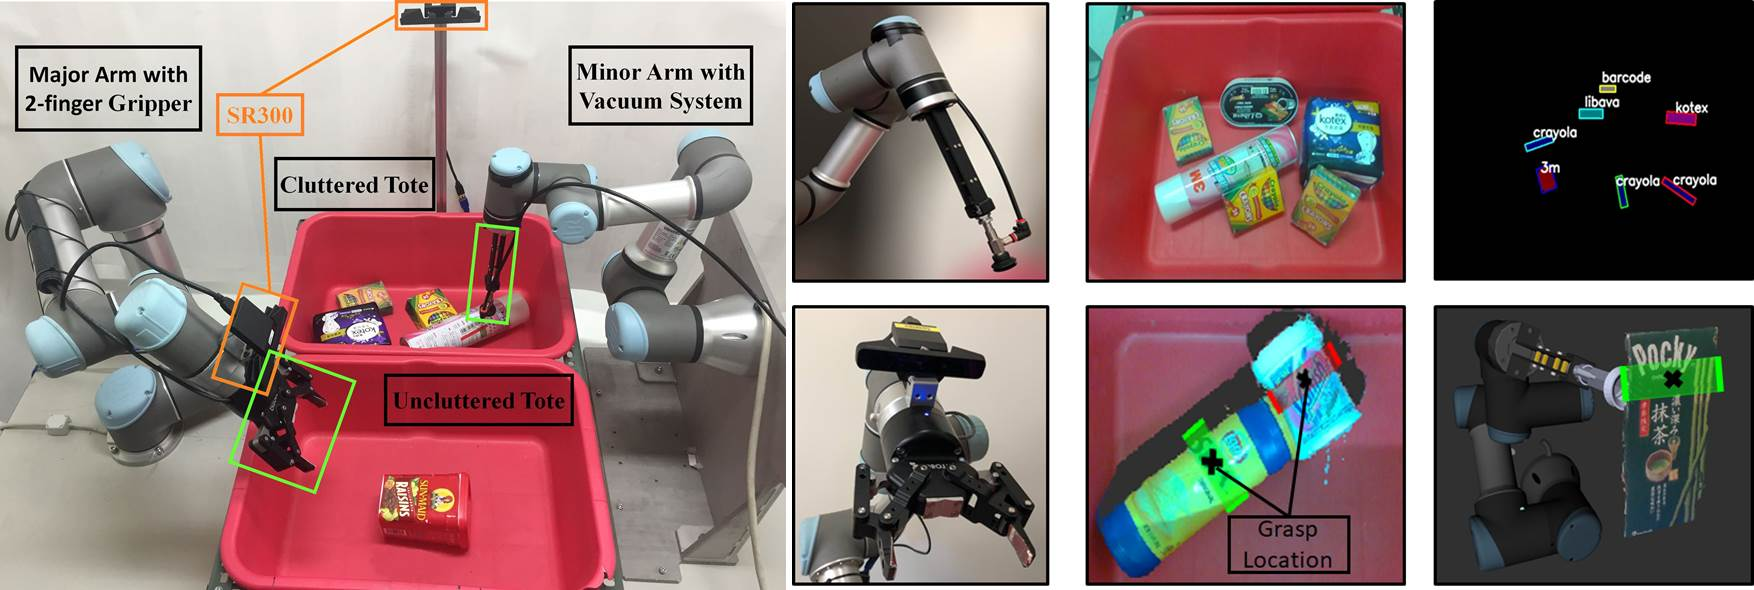
\includegraphics[height=!, width=1.0\linewidth, keepaspectratio=true]
	{./figures/hardware_archi.jpg}
  \caption{圖1.左圖:本研究提出雙手臂主動式操作系統去主動改變場景以達到改善機器人感知環境能力,並最佳化物品夾取可行性系統的效果。吸盤假爪從一個雜亂環境移動物品去取得被隱蔽或部分遮蔽的品牌文字資訊。而雙指假爪則藉由基於品牌文字之線索預測夾取點,以此去完成特定姿態的物品擺放任務。右圖:基於品牌文字,本研究可在雜亂環境中預測品牌文字姿態,並以此針對吸盤假爪與雙指假爪進行物品夾取可能性預測。}
  \label{figure:hardware_archi}
\end{figure}


\subsection{設備介紹}
本研究專注於機器人主動式操作系統,因此手臂、假爪、感測器之選擇十分重要,因此將會逐一分析使用設備之性能以及使用原因。

\paragraph{UR5與UR3協作式機械手臂}
UR5與UR3協作機械手臂乃優傲機械人有限公司(Universal Robots)所生產之協做式機器人,乃六軸機械手臂,其特點為可支援機器人作業系統(Robotic Operation System),適合研究人員快速開發,並擁有安全機制,任意軸碰撞到人或物體,便會自動停止。此外精度都可達至0.1mm,且每軸最快速度可以達到每秒180/360度。UR3/5的活動空間為半徑0.5/0.85m,而承重則分別是3/5 KG,因此本研究所夾取之物品皆低於3公斤以內。考量研究與未來應用之安全性、活動空間以及易開發性,本研究選擇UR5與UR3作為手臂使用。

\begin{figure}[ht]
	\centering
	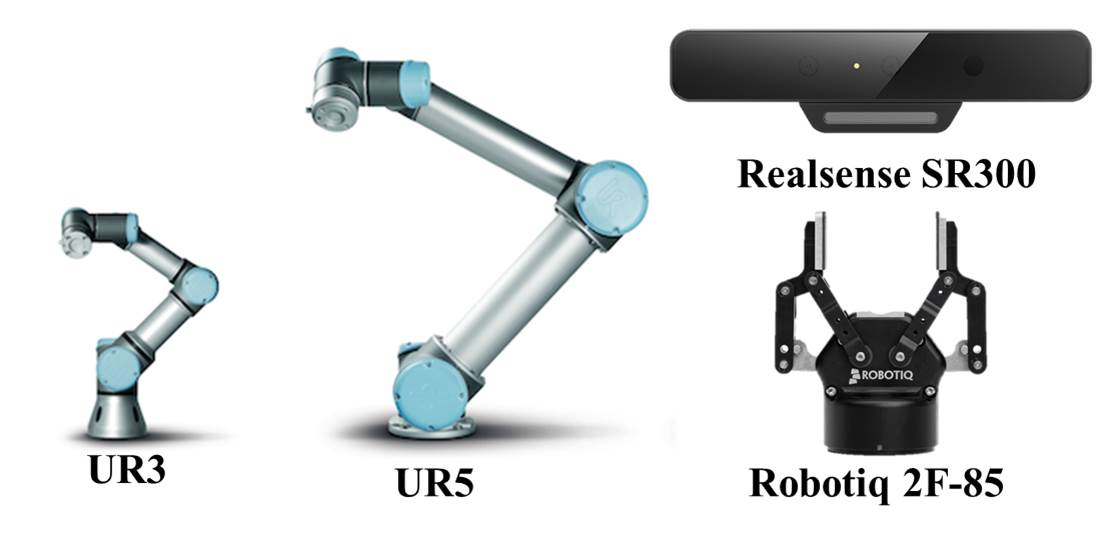
\includegraphics[height=!, width=1.0\linewidth, keepaspectratio=true]
	{./figures/hardware_list.jpg}
  \caption{本研究使用之感測器、機械手臂、假爪。}
  \label{figure:hardware_list}
\end{figure}

\paragraph{Robotiq 2F-85 假爪}
Robotiq 2F-85假爪為機器人公司Robotiq所研發,專門用於機械手臂上的2指假爪。其特色在於其假爪兩指是平行的。並非像人一般是多指靈巧手,雖然變化性較低,卻十分用來夾取形狀簡單的物品。此外此假爪夾取力道可控制從20牛頓至235牛頓,可穩定夾取物品,且重量只有0.9 公斤,並可以裝於UR5末端。它也支援本研究之平台ROS,因此本研究選擇此假爪裝於UR5上,並執行最後特定姿勢的物件夾取與放置任務。

\paragraph{自製吸盤假爪系統}
此系統乃本研究為主動式操作系統特別開發。此系統包含空氣壓縮機、真空產生器、吸盤假爪、以及控制板Arduino UNO。空氣壓縮機乃使用SWAN空氣壓縮機公司之DRS-210-39無油式空壓機,使用壓力可達7 kg/$cm^{2}$,並儲存39公升空氣。而真空產生器則採用MISUMI公司之VJHB6-7,產出之氣壓可達-0.95 kg/$cm^{2}$,且有真空產生、真空破壞等多段式氣壓調整功能。最後搭配自製之吸盤假爪,此吸盤夾爪可裝於UR3上,並補足其工作範圍較小的問題,此外吸盤內徑為0.02cm,搭配真空產生器、空氣壓縮機,垂直作用力可達3 kg,可應付市面上大部分的商品。Arduino UNO作為最簡易的控制開發版,用來控制真空產生器,調整吸盤吸力力道。

\begin{figure}[ht]
	\centering
	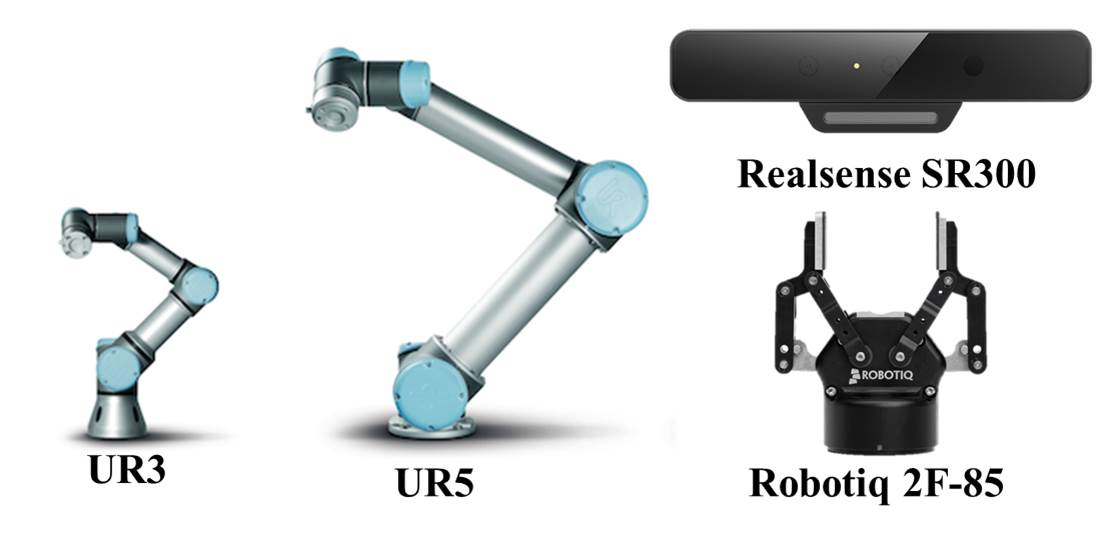
\includegraphics[height=!, width=1.0\linewidth, keepaspectratio=true]
	{./figures/hardware_list.jpg}
  \caption{吸盤假爪系統。}
  \label{figure:suction_gripper}
\end{figure}

\paragraph{RGB-D深度攝影機Realsense SR300}
RGB-D 深度攝影機Realsense SR300乃Intel公司所研發,專用於觀察室內近距離場景,其利用紅外線感知深度,同時具有彩色與深度資訊,操作範圍在0.3 - 2m之間,景深為(H: 73, V: 59, D: 90),且影格率(Frame rate)可達30fps。此感測器雖觀察視野不大,卻能得到視野內非常濃密知點雲資訊,十分適合用於觀測物品點雲,姿態預測用,此外此攝影機也有支援ROS,很適合開發者使用。因此本研究選擇將Realsense SR300安裝於UR5與盒子上,用於觀察物品。

\subsection{多視角主動式視覺}
此系統包含兩個SR300 RGB-D攝影機,一個裝於UR5上,用於控制手臂以改變視角改善感知能力,讓此系統可以解決遮蔽之問題,另一個SR300則裝於桌上並面對雜亂的盒子。

\subsection{手臂假爪配置}
本研究目標為將物品以特定姿態夾取與擺放至架上,考慮物品在雜亂環境中難以一次性以特定姿態去夾取並放置,因此設計不同的假爪給不同的手臂與2階段主動式操作系統:吸盤假爪(UR3)用於第一次夾取,從雜亂環境中夾取至空曠環境,而雙指假爪(UR5)則進行第二次的特定姿態夾取及放置。這樣的設計考量不同假爪的特性:吸盤假爪由於與物品的接觸空間小,容易夾取但移動時不穩定,因此適合用於雜亂環境中的夾取,而雙指假爪則相反,與物品的接觸空間小,夾取物品須有特定姿態,且容易受物體遮蔽影響,但夾取後移動相對穩定,因此用於第二次的夾取。


\section{商品語意資料庫}
就本研究所知,本研究之商品語意基準資料庫為第一個資料庫專注於使用語意標註進行特定姿態放置。有許多相關聯的研究如以場景為單位的Grocery Dataset ~\cite{},此資料集蒐集25類物品並專注於場景中物品的分類,而不是語意切割。以物體為單位之``Shelf & Tote’’資料集,雖也是進行語意標註,但專注於夾取,而不是放置。本研究建立之資料庫包含以物件為單位以及品牌文字、條碼語意為單位之標註,並整理成3大資料集:1. 現實世界訓練資料集:蒐集來自現實,並包含現實環境噪音(亮暗變化、反射)、不同色調的資料。這組訓練集將被用來訓練物品語意切割模型以及品牌文字語意切割模型。2. 虛擬環境訓練資料集:來自虛擬環境Unity,並參考現實世界設定去蒐集。3. 真實世界測試資料集:包含簡單與複雜困難場景,場景中有雜亂、遮頁、複製品狀況發生。這組測試集將被用來比較評估主動式操作與~\cite{peterthesis}之效能。

\subsection{真實世界訓練集}
這部分資料集蒐集的方法參考這份研究~\cite{},這份研究的技術也被應用於Amazon Picking Challenge 2016。每一個場景中,單一物品被隨意放置於盒子中,一個RGB-D攝影機安裝於UR5上,用於可系統的移動手臂並在多個視角自動蒐集資料。本研究選擇20個商品做為目標物品,這些物品皆遵守以下的規則:1. 品牌文字高度皆至少大於1.5cm。 2.品牌文字皆為單行。3. 品牌文字不重複出現於物品上。資料集總共有$920 scenes\times 31 views$。但由於硬體因素,過程中有22張圖片遺漏,因此總共有28,498張圖片。

\paragraph{物體}
\paragraph{品牌文字}

\begin{figure}[ht]
	\centering
	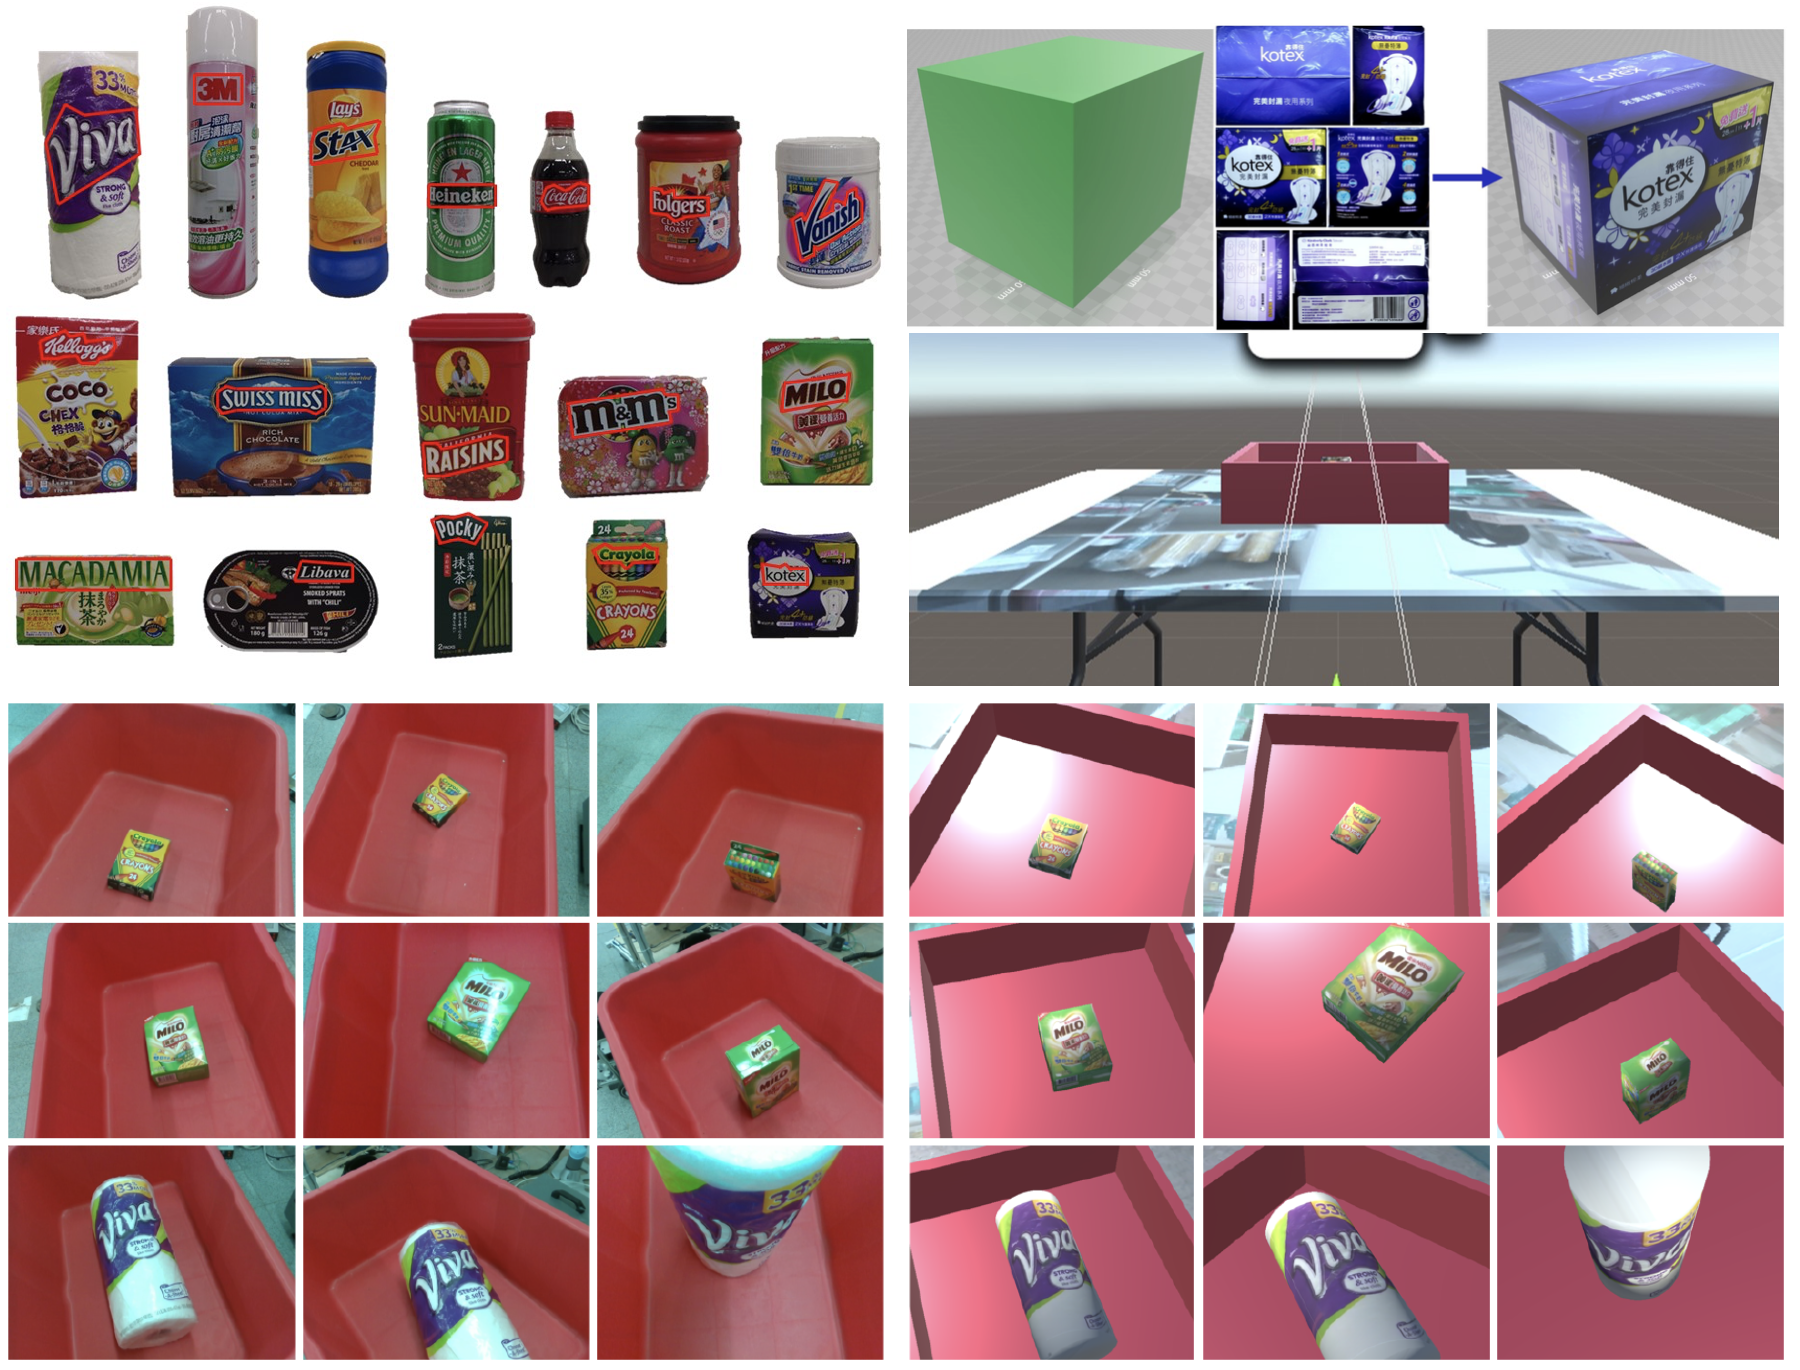
\includegraphics[height=!, width=1.0\linewidth, keepaspectratio=true]
	{./figures/bn-benchmark-dataset.png}
  \caption{於現實(左)與虛擬(右)環境蒐集訓練集。左上:物品範例與品牌文字語意(紅色多邊形框住範圍)。右上:虛擬環境建立示意圖。藉由3D Builder創造物品三維模型,之後建立相似現實環境的紅色盒子於Unity中,並架設相機與物品以蒐集虛擬資料集。蒐集資料時在虛擬與現實的每一個場景中都只有一個物品,這靈感取自~\cite{}說明在單一場景單一物品並利用巨量資料集的訓練語意切割模型之下,在之後多物品場景的情況下仍能得到不錯效果。}
  \label{figure:testset}
\end{figure}


\subsection{虛擬世界訓練集}

\subsection{真實世界測試集}

\begin{figure}[ht]
	\centering
	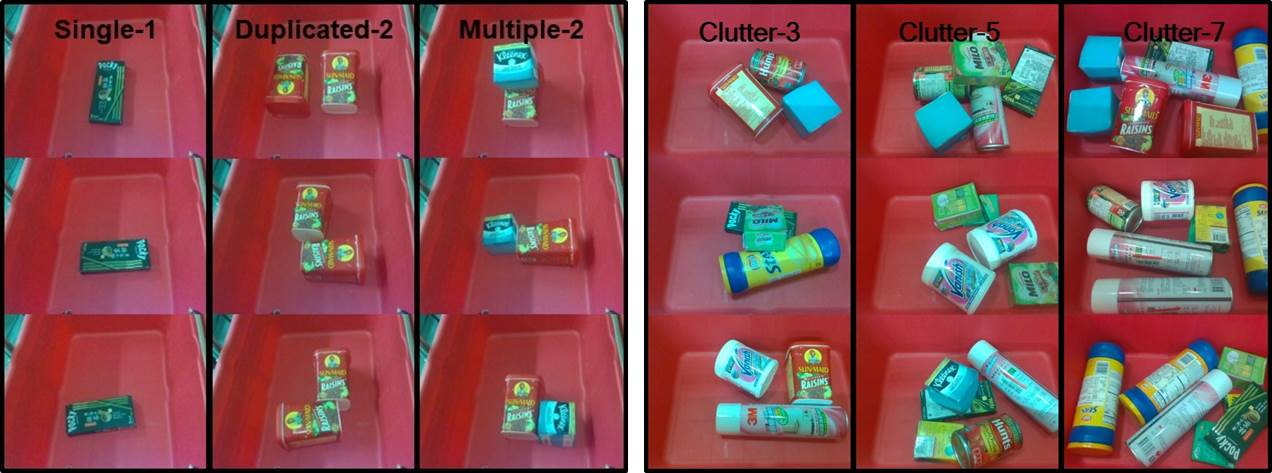
\includegraphics[height=!, width=1.0\linewidth, keepaspectratio=true]
	{./figures/testset.jpg}
  \caption{本研究將測試集分為簡單與複雜場景。在簡單場景中(左)可再細分為Single-1、Duplicated-2、Multiple-2,這3類場景雖會出現相鄰、互相遮蔽情況,但品牌文字皆朝上。而複雜場景中,雜亂程度與遮蔽情況更為明顯,按複雜度分類可再細分為Clutter-3、Clutter-5、Clutter-7,數字代表場景中會出現的物品數量。再這些場景中,物品乃隨意擺置,因此品牌文字可能朝上或朝下看不見。}
  \label{figure:testset}
\end{figure}

\section{基於品牌文字之夾取可行性預測}

\subsection{品牌文字語意分割}

\subsection{夾取可行性預測}

\section{主動式操作系統}

\subsection{單手臂操作}
本研究專注於透過設計資料庫並用其資料訓練夾取可行性預測系統,並以此作為線索作為雙手臂主動式操

\subsection{夾取可行性預測}
本研究專注於透過設計資料庫並用其資料訓練夾取可行性預測系統,並以此作為線索作為雙手臂主動式操
